% Options for packages loaded elsewhere
\PassOptionsToPackage{unicode}{hyperref}
\PassOptionsToPackage{hyphens}{url}
%
\documentclass[
]{article}
\usepackage{amsmath,amssymb}
\usepackage{iftex}
\ifPDFTeX
  \usepackage[T1]{fontenc}
  \usepackage[utf8]{inputenc}
  \usepackage{textcomp} % provide euro and other symbols
\else % if luatex or xetex
  \usepackage{unicode-math} % this also loads fontspec
  \defaultfontfeatures{Scale=MatchLowercase}
  \defaultfontfeatures[\rmfamily]{Ligatures=TeX,Scale=1}
\fi
\usepackage{lmodern}
\ifPDFTeX\else
  % xetex/luatex font selection
\fi
% Use upquote if available, for straight quotes in verbatim environments
\IfFileExists{upquote.sty}{\usepackage{upquote}}{}
\IfFileExists{microtype.sty}{% use microtype if available
  \usepackage[]{microtype}
  \UseMicrotypeSet[protrusion]{basicmath} % disable protrusion for tt fonts
}{}
\makeatletter
\@ifundefined{KOMAClassName}{% if non-KOMA class
  \IfFileExists{parskip.sty}{%
    \usepackage{parskip}
  }{% else
    \setlength{\parindent}{0pt}
    \setlength{\parskip}{6pt plus 2pt minus 1pt}}
}{% if KOMA class
  \KOMAoptions{parskip=half}}
\makeatother
\usepackage{xcolor}
\usepackage[margin=1in]{geometry}
\usepackage{color}
\usepackage{fancyvrb}
\newcommand{\VerbBar}{|}
\newcommand{\VERB}{\Verb[commandchars=\\\{\}]}
\DefineVerbatimEnvironment{Highlighting}{Verbatim}{commandchars=\\\{\}}
% Add ',fontsize=\small' for more characters per line
\usepackage{framed}
\definecolor{shadecolor}{RGB}{248,248,248}
\newenvironment{Shaded}{\begin{snugshade}}{\end{snugshade}}
\newcommand{\AlertTok}[1]{\textcolor[rgb]{0.94,0.16,0.16}{#1}}
\newcommand{\AnnotationTok}[1]{\textcolor[rgb]{0.56,0.35,0.01}{\textbf{\textit{#1}}}}
\newcommand{\AttributeTok}[1]{\textcolor[rgb]{0.13,0.29,0.53}{#1}}
\newcommand{\BaseNTok}[1]{\textcolor[rgb]{0.00,0.00,0.81}{#1}}
\newcommand{\BuiltInTok}[1]{#1}
\newcommand{\CharTok}[1]{\textcolor[rgb]{0.31,0.60,0.02}{#1}}
\newcommand{\CommentTok}[1]{\textcolor[rgb]{0.56,0.35,0.01}{\textit{#1}}}
\newcommand{\CommentVarTok}[1]{\textcolor[rgb]{0.56,0.35,0.01}{\textbf{\textit{#1}}}}
\newcommand{\ConstantTok}[1]{\textcolor[rgb]{0.56,0.35,0.01}{#1}}
\newcommand{\ControlFlowTok}[1]{\textcolor[rgb]{0.13,0.29,0.53}{\textbf{#1}}}
\newcommand{\DataTypeTok}[1]{\textcolor[rgb]{0.13,0.29,0.53}{#1}}
\newcommand{\DecValTok}[1]{\textcolor[rgb]{0.00,0.00,0.81}{#1}}
\newcommand{\DocumentationTok}[1]{\textcolor[rgb]{0.56,0.35,0.01}{\textbf{\textit{#1}}}}
\newcommand{\ErrorTok}[1]{\textcolor[rgb]{0.64,0.00,0.00}{\textbf{#1}}}
\newcommand{\ExtensionTok}[1]{#1}
\newcommand{\FloatTok}[1]{\textcolor[rgb]{0.00,0.00,0.81}{#1}}
\newcommand{\FunctionTok}[1]{\textcolor[rgb]{0.13,0.29,0.53}{\textbf{#1}}}
\newcommand{\ImportTok}[1]{#1}
\newcommand{\InformationTok}[1]{\textcolor[rgb]{0.56,0.35,0.01}{\textbf{\textit{#1}}}}
\newcommand{\KeywordTok}[1]{\textcolor[rgb]{0.13,0.29,0.53}{\textbf{#1}}}
\newcommand{\NormalTok}[1]{#1}
\newcommand{\OperatorTok}[1]{\textcolor[rgb]{0.81,0.36,0.00}{\textbf{#1}}}
\newcommand{\OtherTok}[1]{\textcolor[rgb]{0.56,0.35,0.01}{#1}}
\newcommand{\PreprocessorTok}[1]{\textcolor[rgb]{0.56,0.35,0.01}{\textit{#1}}}
\newcommand{\RegionMarkerTok}[1]{#1}
\newcommand{\SpecialCharTok}[1]{\textcolor[rgb]{0.81,0.36,0.00}{\textbf{#1}}}
\newcommand{\SpecialStringTok}[1]{\textcolor[rgb]{0.31,0.60,0.02}{#1}}
\newcommand{\StringTok}[1]{\textcolor[rgb]{0.31,0.60,0.02}{#1}}
\newcommand{\VariableTok}[1]{\textcolor[rgb]{0.00,0.00,0.00}{#1}}
\newcommand{\VerbatimStringTok}[1]{\textcolor[rgb]{0.31,0.60,0.02}{#1}}
\newcommand{\WarningTok}[1]{\textcolor[rgb]{0.56,0.35,0.01}{\textbf{\textit{#1}}}}
\usepackage{graphicx}
\makeatletter
\def\maxwidth{\ifdim\Gin@nat@width>\linewidth\linewidth\else\Gin@nat@width\fi}
\def\maxheight{\ifdim\Gin@nat@height>\textheight\textheight\else\Gin@nat@height\fi}
\makeatother
% Scale images if necessary, so that they will not overflow the page
% margins by default, and it is still possible to overwrite the defaults
% using explicit options in \includegraphics[width, height, ...]{}
\setkeys{Gin}{width=\maxwidth,height=\maxheight,keepaspectratio}
% Set default figure placement to htbp
\makeatletter
\def\fps@figure{htbp}
\makeatother
\setlength{\emergencystretch}{3em} % prevent overfull lines
\providecommand{\tightlist}{%
  \setlength{\itemsep}{0pt}\setlength{\parskip}{0pt}}
\setcounter{secnumdepth}{-\maxdimen} % remove section numbering
\ifLuaTeX
  \usepackage{selnolig}  % disable illegal ligatures
\fi
\IfFileExists{bookmark.sty}{\usepackage{bookmark}}{\usepackage{hyperref}}
\IfFileExists{xurl.sty}{\usepackage{xurl}}{} % add URL line breaks if available
\urlstyle{same}
\hypersetup{
  pdftitle={Homework Week 7},
  pdfauthor={Retno K. Ningrum},
  hidelinks,
  pdfcreator={LaTeX via pandoc}}

\title{Homework Week 7}
\author{Retno K. Ningrum}
\date{2024-10-09}

\begin{document}
\maketitle

\hypertarget{creating-map-with-r}{%
\section{Creating Map with R}\label{creating-map-with-r}}

This assignment use
\href{https://raw.githubusercontent.com/rfordatascience/tidytuesday/master/data/2021/2021-01-26/plastics.csv}{Plastic
Pollution Dataset} with specific countries in Southeast Asia
(\emph{Indonesia, Singapore, Malaysia, Philippines, Thailand, Vietnam,
Cambodia, Laos, China,Timor-Leste, Myanmar}).

\hypertarget{overall-steps-summary}{%
\subsection{Overall Steps Summary}\label{overall-steps-summary}}

\begin{enumerate}
\def\labelenumi{\arabic{enumi}.}
\tightlist
\item
  Filter data plastic from Southeast Asia (SEA) country and then sum all
  the total plastic in each country
\item
  Filter world data using country mentioned in plastic data in SEA
\item
  Join the plastic data in SEA with the world data
\item
  Create text for each country label manually, following the coordinate
  of each country
\item
  create the plot!
\end{enumerate}

\hypertarget{load-libraries}{%
\subsubsection{Load Libraries}\label{load-libraries}}

load all necessary libraries

\begin{Shaded}
\begin{Highlighting}[]
\FunctionTok{library}\NormalTok{(tidyverse)}
\FunctionTok{library}\NormalTok{(here)}
\FunctionTok{library}\NormalTok{(maps)}
\FunctionTok{library}\NormalTok{(mapdata)}
\FunctionTok{library}\NormalTok{(mapproj)}
\end{Highlighting}
\end{Shaded}

\hypertarget{load-and-inspect-the-data}{%
\subsubsection{Load and Inspect the
Data}\label{load-and-inspect-the-data}}

\begin{Shaded}
\begin{Highlighting}[]
\CommentTok{\#Read the plastic data}
\NormalTok{plastics }\OtherTok{\textless{}{-}}\NormalTok{ readr}\SpecialCharTok{::}\FunctionTok{read\_csv}\NormalTok{(}\StringTok{\textquotesingle{}https://raw.githubusercontent.com/rfordatascience/tidytuesday/master/data/2021/2021{-}01{-}26/plastics.csv\textquotesingle{}}\NormalTok{)}

\CommentTok{\#Read the world data (for mapping)}
\NormalTok{world }\OtherTok{\textless{}{-}} \FunctionTok{map\_data}\NormalTok{(}\StringTok{"world"}\NormalTok{)}

\CommentTok{\#Check the first 10 data}
\FunctionTok{head}\NormalTok{(plastics)}
\end{Highlighting}
\end{Shaded}

\begin{verbatim}
## # A tibble: 6 x 14
##   country    year parent_company empty  hdpe  ldpe     o   pet    pp    ps   pvc
##   <chr>     <dbl> <chr>          <dbl> <dbl> <dbl> <dbl> <dbl> <dbl> <dbl> <dbl>
## 1 Argentina  2019 Grand Total        0   215    55   607  1376   281   116    18
## 2 Argentina  2019 Unbranded          0   155    50   532   848   122   114    17
## 3 Argentina  2019 The Coca-Cola~     0     0     0     0   222    35     0     0
## 4 Argentina  2019 Secco              0     0     0     0    39     4     0     0
## 5 Argentina  2019 Doble Cola         0     0     0     0    38     0     0     0
## 6 Argentina  2019 Pritty             0     0     0     0    22     7     0     0
## # i 3 more variables: grand_total <dbl>, num_events <dbl>, volunteers <dbl>
\end{verbatim}

\begin{Shaded}
\begin{Highlighting}[]
\FunctionTok{head}\NormalTok{(world)}
\end{Highlighting}
\end{Shaded}

\begin{verbatim}
##        long      lat group order region subregion
## 1 -69.89912 12.45200     1     1  Aruba      <NA>
## 2 -69.89571 12.42300     1     2  Aruba      <NA>
## 3 -69.94219 12.43853     1     3  Aruba      <NA>
## 4 -70.00415 12.50049     1     4  Aruba      <NA>
## 5 -70.06612 12.54697     1     5  Aruba      <NA>
## 6 -70.05088 12.59707     1     6  Aruba      <NA>
\end{verbatim}

\begin{Shaded}
\begin{Highlighting}[]
\CommentTok{\#check overall data}
\FunctionTok{glimpse}\NormalTok{(plastics)}
\end{Highlighting}
\end{Shaded}

\begin{verbatim}
## Rows: 13,380
## Columns: 14
## $ country        <chr> "Argentina", "Argentina", "Argentina", "Argentina", "Ar~
## $ year           <dbl> 2019, 2019, 2019, 2019, 2019, 2019, 2019, 2019, 2019, 2~
## $ parent_company <chr> "Grand Total", "Unbranded", "The Coca-Cola Company", "S~
## $ empty          <dbl> 0, 0, 0, 0, 0, 0, 0, 0, 0, 0, 0, 0, 0, 0, 0, 0, 0, 0, 0~
## $ hdpe           <dbl> 215, 155, 0, 0, 0, 0, 0, 0, 0, 0, 0, 0, 0, 0, 0, 0, 0, ~
## $ ldpe           <dbl> 55, 50, 0, 0, 0, 0, 0, 0, 0, 0, 0, 0, 0, 0, 0, 0, 0, 0,~
## $ o              <dbl> 607, 532, 0, 0, 0, 0, 0, 0, 0, 0, 0, 0, 0, 13, 0, 0, 0,~
## $ pet            <dbl> 1376, 848, 222, 39, 38, 22, 21, 26, 19, 14, 14, 14, 14,~
## $ pp             <dbl> 281, 122, 35, 4, 0, 7, 6, 0, 1, 4, 3, 1, 0, 0, 3, 0, 4,~
## $ ps             <dbl> 116, 114, 0, 0, 0, 0, 0, 0, 0, 0, 0, 0, 0, 0, 0, 0, 0, ~
## $ pvc            <dbl> 18, 17, 0, 0, 0, 0, 0, 0, 0, 0, 0, 0, 0, 0, 0, 0, 0, 0,~
## $ grand_total    <dbl> 2668, 1838, 257, 43, 38, 29, 27, 26, 20, 18, 17, 15, 14~
## $ num_events     <dbl> 4, 4, 4, 4, 4, 4, 4, 4, 4, 4, 4, 4, 4, 4, 4, 4, 4, 4, 4~
## $ volunteers     <dbl> 243, 243, 243, 243, 243, 243, 243, 243, 243, 243, 243, ~
\end{verbatim}

\begin{Shaded}
\begin{Highlighting}[]
\FunctionTok{glimpse}\NormalTok{(world)}
\end{Highlighting}
\end{Shaded}

\begin{verbatim}
## Rows: 99,338
## Columns: 6
## $ long      <dbl> -69.89912, -69.89571, -69.94219, -70.00415, -70.06612, -70.0~
## $ lat       <dbl> 12.45200, 12.42300, 12.43853, 12.50049, 12.54697, 12.59707, ~
## $ group     <dbl> 1, 1, 1, 1, 1, 1, 1, 1, 1, 1, 2, 2, 2, 2, 2, 2, 2, 2, 2, 2, ~
## $ order     <int> 1, 2, 3, 4, 5, 6, 7, 8, 9, 10, 12, 13, 14, 15, 16, 17, 18, 1~
## $ region    <chr> "Aruba", "Aruba", "Aruba", "Aruba", "Aruba", "Aruba", "Aruba~
## $ subregion <chr> NA, NA, NA, NA, NA, NA, NA, NA, NA, NA, NA, NA, NA, NA, NA, ~
\end{verbatim}

\begin{Shaded}
\begin{Highlighting}[]
\FunctionTok{unique}\NormalTok{(plastics}\SpecialCharTok{$}\NormalTok{country)  }\CommentTok{\#to check the list of country covered in the plastics data}
\end{Highlighting}
\end{Shaded}

\begin{verbatim}
##  [1] "Argentina"                                         
##  [2] "Australia"                                         
##  [3] "Bangladesh"                                        
##  [4] "Benin"                                             
##  [5] "Bhutan"                                            
##  [6] "Brazil"                                            
##  [7] "Bulgaria"                                          
##  [8] "Burkina Faso"                                      
##  [9] "Cameroon"                                          
## [10] "Canada"                                            
## [11] "China"                                             
## [12] "Colombia"                                          
## [13] "Cote D_ivoire"                                     
## [14] "Cyprus"                                            
## [15] "ECUADOR"                                           
## [16] "EMPTY"                                             
## [17] "France"                                            
## [18] "Germany"                                           
## [19] "Ghana"                                             
## [20] "Hong Kong"                                         
## [21] "India"                                             
## [22] "Indonesia"                                         
## [23] "Ireland"                                           
## [24] "Italy"                                             
## [25] "Japan"                                             
## [26] "Kenya"                                             
## [27] "Latvia"                                            
## [28] "Luxembourg"                                        
## [29] "Malaysia"                                          
## [30] "Maldives"                                          
## [31] "Mexico"                                            
## [32] "Montenegro"                                        
## [33] "NIGERIA"                                           
## [34] "Netherlands"                                       
## [35] "Philippines"                                       
## [36] "Portugal"                                          
## [37] "Rwanda"                                            
## [38] "Slovenia"                                          
## [39] "South Africa"                                      
## [40] "Spain"                                             
## [41] "Sri Lanka"                                         
## [42] "Switzerland"                                       
## [43] "Taiwan_ Republic of China (ROC)"                   
## [44] "Tanzania"                                          
## [45] "Thailand"                                          
## [46] "Tunisia"                                           
## [47] "Turkey"                                            
## [48] "Ukraine"                                           
## [49] "United Arab Emirates"                              
## [50] "United Kingdom"                                    
## [51] "United States of America"                          
## [52] "Vietnam"                                           
## [53] "Armenia"                                           
## [54] "Chile"                                             
## [55] "Denmark"                                           
## [56] "Ecuador"                                           
## [57] "El Salvador"                                       
## [58] "Greece"                                            
## [59] "Honduras"                                          
## [60] "Korea"                                             
## [61] "Kuwait"                                            
## [62] "Lithuania"                                         
## [63] "Nigeria"                                           
## [64] "Peru"                                              
## [65] "Romania"                                           
## [66] "Serbia"                                            
## [67] "Singapore"                                         
## [68] "Togo"                                              
## [69] "United Kingdom of Great Britain & Northern Ireland"
\end{verbatim}

\begin{Shaded}
\begin{Highlighting}[]
\FunctionTok{unique}\NormalTok{(world}\SpecialCharTok{$}\NormalTok{region)      }\CommentTok{\#to check the list of country covered in the world data}
\end{Highlighting}
\end{Shaded}

\begin{verbatim}
##   [1] "Aruba"                              
##   [2] "Afghanistan"                        
##   [3] "Angola"                             
##   [4] "Anguilla"                           
##   [5] "Albania"                            
##   [6] "Finland"                            
##   [7] "Andorra"                            
##   [8] "United Arab Emirates"               
##   [9] "Argentina"                          
##  [10] "Armenia"                            
##  [11] "American Samoa"                     
##  [12] "Antarctica"                         
##  [13] "Australia"                          
##  [14] "French Southern and Antarctic Lands"
##  [15] "Antigua"                            
##  [16] "Barbuda"                            
##  [17] "Austria"                            
##  [18] "Azerbaijan"                         
##  [19] "Burundi"                            
##  [20] "Belgium"                            
##  [21] "Benin"                              
##  [22] "Burkina Faso"                       
##  [23] "Bangladesh"                         
##  [24] "Bulgaria"                           
##  [25] "Bahrain"                            
##  [26] "Bahamas"                            
##  [27] "Bosnia and Herzegovina"             
##  [28] "Saint Barthelemy"                   
##  [29] "Belarus"                            
##  [30] "Belize"                             
##  [31] "Bermuda"                            
##  [32] "Bolivia"                            
##  [33] "Brazil"                             
##  [34] "Barbados"                           
##  [35] "Brunei"                             
##  [36] "Bhutan"                             
##  [37] "Botswana"                           
##  [38] "Central African Republic"           
##  [39] "Canada"                             
##  [40] "Switzerland"                        
##  [41] "Chile"                              
##  [42] "China"                              
##  [43] "Ivory Coast"                        
##  [44] "Cameroon"                           
##  [45] "Democratic Republic of the Congo"   
##  [46] "Republic of Congo"                  
##  [47] "Cook Islands"                       
##  [48] "Colombia"                           
##  [49] "Comoros"                            
##  [50] "Cape Verde"                         
##  [51] "Costa Rica"                         
##  [52] "Cuba"                               
##  [53] "Curacao"                            
##  [54] "Cayman Islands"                     
##  [55] "Cyprus"                             
##  [56] "Czech Republic"                     
##  [57] "Germany"                            
##  [58] "Djibouti"                           
##  [59] "Dominica"                           
##  [60] "Denmark"                            
##  [61] "Dominican Republic"                 
##  [62] "Algeria"                            
##  [63] "Ecuador"                            
##  [64] "Egypt"                              
##  [65] "Eritrea"                            
##  [66] "Canary Islands"                     
##  [67] "Spain"                              
##  [68] "Estonia"                            
##  [69] "Ethiopia"                           
##  [70] "Fiji"                               
##  [71] "Falkland Islands"                   
##  [72] "Reunion"                            
##  [73] "Mayotte"                            
##  [74] "French Guiana"                      
##  [75] "Martinique"                         
##  [76] "Guadeloupe"                         
##  [77] "France"                             
##  [78] "Faroe Islands"                      
##  [79] "Micronesia"                         
##  [80] "Gabon"                              
##  [81] "UK"                                 
##  [82] "Georgia"                            
##  [83] "Guernsey"                           
##  [84] "Ghana"                              
##  [85] "Guinea"                             
##  [86] "Gambia"                             
##  [87] "Guinea-Bissau"                      
##  [88] "Equatorial Guinea"                  
##  [89] "Greece"                             
##  [90] "Grenada"                            
##  [91] "Greenland"                          
##  [92] "Guatemala"                          
##  [93] "Guam"                               
##  [94] "Guyana"                             
##  [95] "Heard Island"                       
##  [96] "Honduras"                           
##  [97] "Croatia"                            
##  [98] "Haiti"                              
##  [99] "Hungary"                            
## [100] "Indonesia"                          
## [101] "Isle of Man"                        
## [102] "India"                              
## [103] "Cocos Islands"                      
## [104] "Christmas Island"                   
## [105] "Chagos Archipelago"                 
## [106] "Ireland"                            
## [107] "Iran"                               
## [108] "Iraq"                               
## [109] "Iceland"                            
## [110] "Israel"                             
## [111] "Italy"                              
## [112] "San Marino"                         
## [113] "Jamaica"                            
## [114] "Jersey"                             
## [115] "Jordan"                             
## [116] "Japan"                              
## [117] "Siachen Glacier"                    
## [118] "Kazakhstan"                         
## [119] "Kenya"                              
## [120] "Kyrgyzstan"                         
## [121] "Cambodia"                           
## [122] "Kiribati"                           
## [123] "Nevis"                              
## [124] "Saint Kitts"                        
## [125] "South Korea"                        
## [126] "Kosovo"                             
## [127] "Kuwait"                             
## [128] "Laos"                               
## [129] "Lebanon"                            
## [130] "Liberia"                            
## [131] "Libya"                              
## [132] "Saint Lucia"                        
## [133] "Liechtenstein"                      
## [134] "Sri Lanka"                          
## [135] "Lesotho"                            
## [136] "Lithuania"                          
## [137] "Luxembourg"                         
## [138] "Latvia"                             
## [139] "Saint Martin"                       
## [140] "Morocco"                            
## [141] "Monaco"                             
## [142] "Moldova"                            
## [143] "Madagascar"                         
## [144] "Maldives"                           
## [145] "Mexico"                             
## [146] "Marshall Islands"                   
## [147] "North Macedonia"                    
## [148] "Mali"                               
## [149] "Malta"                              
## [150] "Myanmar"                            
## [151] "Montenegro"                         
## [152] "Mongolia"                           
## [153] "Northern Mariana Islands"           
## [154] "Mozambique"                         
## [155] "Mauritania"                         
## [156] "Montserrat"                         
## [157] "Mauritius"                          
## [158] "Malawi"                             
## [159] "Malaysia"                           
## [160] "Namibia"                            
## [161] "New Caledonia"                      
## [162] "Niger"                              
## [163] "Norfolk Island"                     
## [164] "Nigeria"                            
## [165] "Nicaragua"                          
## [166] "Niue"                               
## [167] "Bonaire"                            
## [168] "Sint Eustatius"                     
## [169] "Saba"                               
## [170] "Netherlands"                        
## [171] "Norway"                             
## [172] "Nepal"                              
## [173] "Nauru"                              
## [174] "New Zealand"                        
## [175] "Oman"                               
## [176] "Pakistan"                           
## [177] "Panama"                             
## [178] "Pitcairn Islands"                   
## [179] "Peru"                               
## [180] "Philippines"                        
## [181] "Palau"                              
## [182] "Papua New Guinea"                   
## [183] "Poland"                             
## [184] "Puerto Rico"                        
## [185] "North Korea"                        
## [186] "Madeira Islands"                    
## [187] "Azores"                             
## [188] "Portugal"                           
## [189] "Paraguay"                           
## [190] "Palestine"                          
## [191] "French Polynesia"                   
## [192] "Qatar"                              
## [193] "Romania"                            
## [194] "Russia"                             
## [195] "Rwanda"                             
## [196] "Western Sahara"                     
## [197] "Saudi Arabia"                       
## [198] "Sudan"                              
## [199] "South Sudan"                        
## [200] "Senegal"                            
## [201] "Singapore"                          
## [202] "South Sandwich Islands"             
## [203] "South Georgia"                      
## [204] "Saint Helena"                       
## [205] "Ascension Island"                   
## [206] "Solomon Islands"                    
## [207] "Sierra Leone"                       
## [208] "El Salvador"                        
## [209] "Somalia"                            
## [210] "Saint Pierre and Miquelon"          
## [211] "Serbia"                             
## [212] "Sao Tome and Principe"              
## [213] "Suriname"                           
## [214] "Slovakia"                           
## [215] "Slovenia"                           
## [216] "Sweden"                             
## [217] "Swaziland"                          
## [218] "Sint Maarten"                       
## [219] "Seychelles"                         
## [220] "Syria"                              
## [221] "Turks and Caicos Islands"           
## [222] "Chad"                               
## [223] "Togo"                               
## [224] "Thailand"                           
## [225] "Tajikistan"                         
## [226] "Turkmenistan"                       
## [227] "Timor-Leste"                        
## [228] "Tonga"                              
## [229] "Trinidad"                           
## [230] "Tobago"                             
## [231] "Tunisia"                            
## [232] "Turkey"                             
## [233] "Taiwan"                             
## [234] "Tanzania"                           
## [235] "Uganda"                             
## [236] "Ukraine"                            
## [237] "Uruguay"                            
## [238] "USA"                                
## [239] "Uzbekistan"                         
## [240] "Vatican"                            
## [241] "Grenadines"                         
## [242] "Saint Vincent"                      
## [243] "Venezuela"                          
## [244] "Virgin Islands"                     
## [245] "Vietnam"                            
## [246] "Vanuatu"                            
## [247] "Wallis and Futuna"                  
## [248] "Samoa"                              
## [249] "Yemen"                              
## [250] "South Africa"                       
## [251] "Zambia"                             
## [252] "Zimbabwe"
\end{verbatim}

After checking the dataset, I decide to focus on creating map of plastic
distribution in Southeast Asia

\hypertarget{data-cleaning}{%
\subsubsection{Data Cleaning}\label{data-cleaning}}

\begin{Shaded}
\begin{Highlighting}[]
\CommentTok{\#create the SouthEast Asia (SEA) dataset for map background}
\NormalTok{SEA }\OtherTok{\textless{}{-}}\NormalTok{ world }\SpecialCharTok{\%\textgreater{}\%}                                                    \CommentTok{\#use world data}
  \FunctionTok{filter}\NormalTok{(region }\SpecialCharTok{\%in\%} \FunctionTok{c}\NormalTok{(}\StringTok{"Indonesia"}\NormalTok{, }\StringTok{"Singapore"}\NormalTok{, }\StringTok{"Malaysia"}\NormalTok{,        }\CommentTok{\#filter data in region column}
                       \StringTok{"Philippines"}\NormalTok{, }\StringTok{"Thailand"}\NormalTok{, }\StringTok{"Vietnam"}\NormalTok{, }
                       \StringTok{"Cambodia"}\NormalTok{, }\StringTok{"Laos"}\NormalTok{, }\StringTok{"China"}\NormalTok{, }\StringTok{"Timor{-}Leste"}\NormalTok{, }
                       \StringTok{"Myanmar"}\NormalTok{)) }\SpecialCharTok{\%\textgreater{}\%}
  \FunctionTok{select}\NormalTok{(long, lat, group, region)                          }\CommentTok{\#select only long, lat, group, region column}


\CommentTok{\#create the plastic data in SEA}
\NormalTok{plastic\_SEA }\OtherTok{\textless{}{-}}\NormalTok{ plastics }\SpecialCharTok{\%\textgreater{}\%}                          \CommentTok{\#use plastic data}
  \FunctionTok{filter}\NormalTok{(country }\SpecialCharTok{\%in\%} \FunctionTok{c}\NormalTok{(}\StringTok{"Indonesia"}\NormalTok{, }\StringTok{"Singapore"}\NormalTok{,    }\CommentTok{\#filter country in SEA}
                        \StringTok{"Malaysia"}\NormalTok{, }\StringTok{"Philippines"}\NormalTok{, }
                        \StringTok{"Thailand"}\NormalTok{, }\StringTok{"Vietnam"}\NormalTok{)) }\SpecialCharTok{\%\textgreater{}\%}          
  \FunctionTok{select}\NormalTok{(}\StringTok{"region"} \OtherTok{=}\NormalTok{ country,  }\CommentTok{\#Select the country column, but rename it to "region" {-}\textgreater{} for join purposes}
\NormalTok{         grand\_total) }\SpecialCharTok{\%\textgreater{}\%}     \CommentTok{\#select the grand\_total value    }
  \FunctionTok{group\_by}\NormalTok{(region)  }\SpecialCharTok{\%\textgreater{}\%}       \CommentTok{\#group by region}
  \FunctionTok{summarise}\NormalTok{(}\AttributeTok{total\_plastics =} \FunctionTok{sum}\NormalTok{(grand\_total))  }\CommentTok{\#summarize grand\_total in each country/region}

\CommentTok{\#Join the plastic in SEA with SEA}
\NormalTok{SEA\_plastic }\OtherTok{\textless{}{-}} \FunctionTok{left\_join}\NormalTok{(SEA, plastic\_SEA)}

\CommentTok{\#Create label for the map}
\NormalTok{country\_labels }\OtherTok{\textless{}{-}} \FunctionTok{data.frame}\NormalTok{(}
  \AttributeTok{region =} \FunctionTok{c}\NormalTok{(}\StringTok{"Indonesia"}\NormalTok{, }\StringTok{"Malaysia"}\NormalTok{, }\StringTok{"Philippines"}\NormalTok{,  }\CommentTok{\#show the label for these countries}
             \StringTok{"Singapore"}\NormalTok{, }\StringTok{"Thailand"}\NormalTok{, }\StringTok{"Vietnam"}\NormalTok{),}
  \AttributeTok{long =} \FunctionTok{c}\NormalTok{(}\FloatTok{113.9213}\NormalTok{, }\FloatTok{101.9758}\NormalTok{, }\FloatTok{122.5583}\NormalTok{, }\FloatTok{103.8198}\NormalTok{, }\FloatTok{100.9925}\NormalTok{, }\FloatTok{105.8562}\NormalTok{), }\CommentTok{\# set longitudes of each country label}
  \AttributeTok{lat =} \FunctionTok{c}\NormalTok{(}\SpecialCharTok{{-}}\FloatTok{0.7893}\NormalTok{, }\FloatTok{4.2105}\NormalTok{, }\FloatTok{12.8797}\NormalTok{, }\FloatTok{1.3521}\NormalTok{, }\FloatTok{15.8700}\NormalTok{, }\FloatTok{14.0583}\NormalTok{)        }\CommentTok{\# set latitude if each country label}
\NormalTok{)}
\end{Highlighting}
\end{Shaded}

\hypertarget{plot-the-map}{%
\subsubsection{Plot the Map!}\label{plot-the-map}}

\begin{Shaded}
\begin{Highlighting}[]
\CommentTok{\# Plot the map}
\FunctionTok{ggplot}\NormalTok{(}\AttributeTok{data =}\NormalTok{ SEA\_plastic) }\SpecialCharTok{+}                          \CommentTok{\#use data world\_indo as the plot background}
  \FunctionTok{geom\_polygon}\NormalTok{(}\FunctionTok{aes}\NormalTok{(}\AttributeTok{x =}\NormalTok{ long, }\AttributeTok{y =}\NormalTok{ lat,                 }\CommentTok{\#create polygon using x.y coordinate}
                   \AttributeTok{group =}\NormalTok{ group,                     }\CommentTok{\#group by group}
                   \AttributeTok{fill =}\NormalTok{ total\_plastics),            }\CommentTok{\#fill data using total\_plastics}
               \AttributeTok{color =} \StringTok{"white"}\NormalTok{) }\SpecialCharTok{+}                     \CommentTok{\#country border is white}
  \FunctionTok{geom\_text}\NormalTok{(}\AttributeTok{data =}\NormalTok{ country\_labels,                    }\CommentTok{\#use data from country\_labels}
            \FunctionTok{aes}\NormalTok{(}\AttributeTok{x =}\NormalTok{ long, }\AttributeTok{y =}\NormalTok{ lat,                    }\CommentTok{\#set text by long and lat axis}
                \AttributeTok{label =}\NormalTok{ region),                      }\CommentTok{\#label text by region}
            \AttributeTok{size =} \FloatTok{3.5}\NormalTok{,  }\AttributeTok{color =} \StringTok{"black"}\NormalTok{) }\SpecialCharTok{+}           \CommentTok{\#set the size by 3.5, text color is black}
  \FunctionTok{coord\_map}\NormalTok{(}\AttributeTok{projection =} \StringTok{"mercator"}\NormalTok{, }\CommentTok{\#Use the mercator type as projected map}
            \AttributeTok{xlim =} \FunctionTok{c}\NormalTok{(}\DecValTok{95}\NormalTok{, }\DecValTok{139}\NormalTok{),       }\CommentTok{\#set the x coordinate from 95 to 139 (this is indonesia coordinate) }
            \AttributeTok{ylim =} \FunctionTok{c}\NormalTok{(}\SpecialCharTok{{-}}\DecValTok{10}\NormalTok{, }\DecValTok{21}\NormalTok{)) }\SpecialCharTok{+}     \CommentTok{\#set the y coordinate from {-}10 to 12 (this is indonesia coordinate)}
  \FunctionTok{labs}\NormalTok{(}\AttributeTok{title =} \StringTok{"Plastic Distribution in Southeast Asia"}\NormalTok{,  }\CommentTok{\#Add title}
       \AttributeTok{subtitle =} \StringTok{"Indonesia, Singapore, Malaysia, Philippines, Thailand, Vietnam"}\NormalTok{,   }\CommentTok{\#Add subtitle}
       \AttributeTok{x =} \StringTok{"Longitude"}\NormalTok{,                                   }\CommentTok{\#Add X{-}axis label}
       \AttributeTok{y =} \StringTok{"Latitude"}\NormalTok{) }\SpecialCharTok{+}                                  \CommentTok{\#Add Y{-}axis label}
  \FunctionTok{theme\_minimal}\NormalTok{() }\SpecialCharTok{+}                                       \CommentTok{\#Apply minimal theme for clean appearance}
  \FunctionTok{theme}\NormalTok{(}\AttributeTok{panel.grid.major =} \FunctionTok{element\_line}\NormalTok{(}\AttributeTok{color =} \StringTok{"gray"}\NormalTok{,       }\CommentTok{\#Add gridline, color grey}
                                        \AttributeTok{linetype =} \StringTok{"dotted"}\NormalTok{), }\CommentTok{\#set type of gridline: dotted gridline}
        \AttributeTok{plot.title =} \FunctionTok{element\_text}\NormalTok{(}\AttributeTok{hjust =} \FloatTok{0.5}\NormalTok{,     }\CommentTok{\#place the title text in the center}
                                  \AttributeTok{size =} \DecValTok{16}\NormalTok{,       }\CommentTok{\#Set font size = 16}
                                  \AttributeTok{face =} \StringTok{"bold"}\NormalTok{),}
        \AttributeTok{plot.subtitle =} \FunctionTok{element\_text}\NormalTok{(}\AttributeTok{hjust =} \FloatTok{0.5}\NormalTok{,  }\CommentTok{\#place the subtitle text in the center}
                                  \AttributeTok{size =} \DecValTok{12}\NormalTok{ ))     }\CommentTok{\#Set font size = 12}
\end{Highlighting}
\end{Shaded}

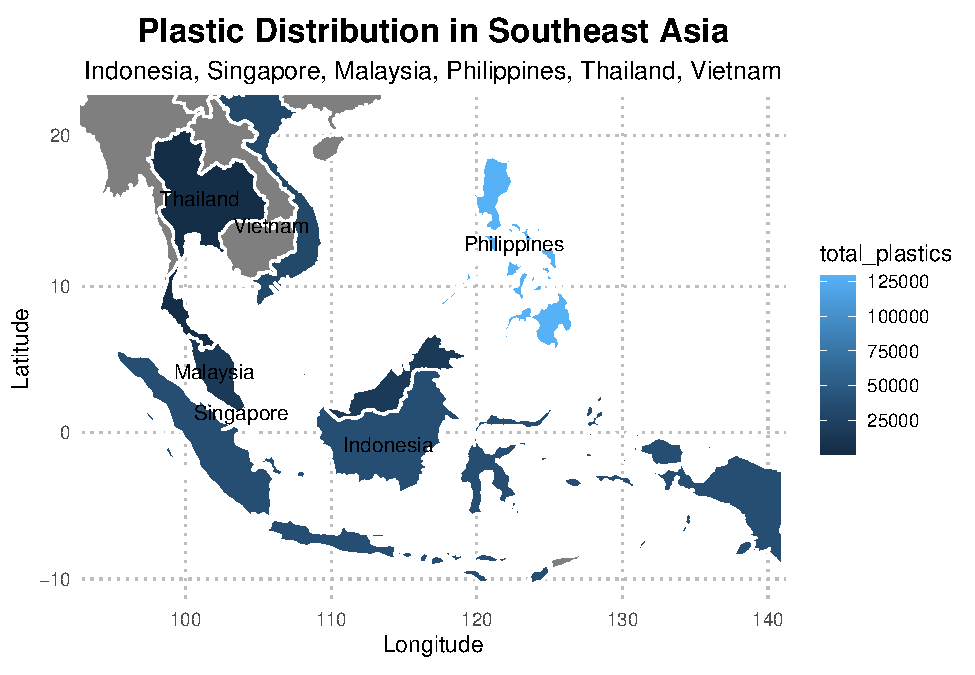
\includegraphics{../output/plastic_SEA-1.pdf}

\end{document}
